\documentclass[twoside]{book}

% Packages required by doxygen
\usepackage{calc}
\usepackage{doxygen}
\usepackage{graphicx}
\usepackage[utf8]{inputenc}
\usepackage{makeidx}
\usepackage{multicol}
\usepackage{multirow}
\usepackage{textcomp}
\usepackage[table]{xcolor}

% Font selection
\usepackage[T1]{fontenc}
\usepackage{mathptmx}
\usepackage[scaled=.90]{helvet}
\usepackage{courier}
\usepackage{amssymb}
\usepackage{sectsty}
\renewcommand{\familydefault}{\sfdefault}
\allsectionsfont{%
  \fontseries{bc}\selectfont%
  \color{darkgray}%
}
\renewcommand{\DoxyLabelFont}{%
  \fontseries{bc}\selectfont%
  \color{darkgray}%
}

% Page & text layout
\usepackage{geometry}
\geometry{%
  a4paper,%
  top=2.5cm,%
  bottom=2.5cm,%
  left=2.5cm,%
  right=2.5cm%
}
\tolerance=750
\hfuzz=15pt
\hbadness=750
\setlength{\emergencystretch}{15pt}
\setlength{\parindent}{0cm}
\setlength{\parskip}{0.2cm}
\makeatletter
\renewcommand{\paragraph}{%
  \@startsection{paragraph}{4}{0ex}{-1.0ex}{1.0ex}{%
    \normalfont\normalsize\bfseries\SS@parafont%
  }%
}
\renewcommand{\subparagraph}{%
  \@startsection{subparagraph}{5}{0ex}{-1.0ex}{1.0ex}{%
    \normalfont\normalsize\bfseries\SS@subparafont%
  }%
}
\makeatother

% Headers & footers
\usepackage{fancyhdr}
\pagestyle{fancyplain}
\fancyhead[LE]{\fancyplain{}{\bfseries\thepage}}
\fancyhead[CE]{\fancyplain{}{}}
\fancyhead[RE]{\fancyplain{}{\bfseries\leftmark}}
\fancyhead[LO]{\fancyplain{}{\bfseries\rightmark}}
\fancyhead[CO]{\fancyplain{}{}}
\fancyhead[RO]{\fancyplain{}{\bfseries\thepage}}
\fancyfoot[LE]{\fancyplain{}{}}
\fancyfoot[CE]{\fancyplain{}{}}
\fancyfoot[RE]{\fancyplain{}{\bfseries\scriptsize Generated on Tue Oct 20 2015 18\-:40\-:17 for My Project by Doxygen }}
\fancyfoot[LO]{\fancyplain{}{\bfseries\scriptsize Generated on Tue Oct 20 2015 18\-:40\-:17 for My Project by Doxygen }}
\fancyfoot[CO]{\fancyplain{}{}}
\fancyfoot[RO]{\fancyplain{}{}}
\renewcommand{\footrulewidth}{0.4pt}
\renewcommand{\chaptermark}[1]{%
  \markboth{#1}{}%
}
\renewcommand{\sectionmark}[1]{%
  \markright{\thesection\ #1}%
}

% Indices & bibliography
\usepackage{natbib}
\usepackage[titles]{tocloft}
\setcounter{tocdepth}{3}
\setcounter{secnumdepth}{5}
\makeindex

% Hyperlinks (required, but should be loaded last)
\usepackage{ifpdf}
\ifpdf
  \usepackage[pdftex,pagebackref=true]{hyperref}
\else
  \usepackage[ps2pdf,pagebackref=true]{hyperref}
\fi
\hypersetup{%
  colorlinks=true,%
  linkcolor=blue,%
  citecolor=blue,%
  unicode%
}

% Custom commands
\newcommand{\clearemptydoublepage}{%
  \newpage{\pagestyle{empty}\cleardoublepage}%
}


%===== C O N T E N T S =====

\begin{document}

% Titlepage & ToC
\hypersetup{pageanchor=false}
\pagenumbering{roman}
\begin{titlepage}
\vspace*{7cm}
\begin{center}%
{\Large My Project }\\
\vspace*{1cm}
{\large Generated by Doxygen 1.8.6}\\
\vspace*{0.5cm}
{\small Tue Oct 20 2015 18:40:17}\\
\end{center}
\end{titlepage}
\clearemptydoublepage
\tableofcontents
\clearemptydoublepage
\pagenumbering{arabic}
\hypersetup{pageanchor=true}

%--- Begin generated contents ---
\chapter{cs371p-\/allocator}
\label{md_README}
\hypertarget{md_README}{}
Time to complete is estimated at 18 hours 
\chapter{Hierarchical Index}
\section{Class Hierarchy}
This inheritance list is sorted roughly, but not completely, alphabetically\-:\begin{DoxyCompactList}
\item \contentsline{section}{Allocator$<$ T, N $>$}{\pageref{classAllocator}}{}
\item Test\begin{DoxyCompactList}
\item \contentsline{section}{Test\-Allocator1$<$ A $>$}{\pageref{structTestAllocator1}}{}
\item \contentsline{section}{Test\-Allocator3$<$ A $>$}{\pageref{structTestAllocator3}}{}
\end{DoxyCompactList}
\end{DoxyCompactList}

\chapter{Class Index}
\section{Class List}
Here are the classes, structs, unions and interfaces with brief descriptions\-:\begin{DoxyCompactList}
\item\contentsline{section}{\hyperlink{classAllocator}{Allocator$<$ T, N $>$} }{\pageref{classAllocator}}{}
\item\contentsline{section}{\hyperlink{structTestAllocator1}{Test\-Allocator1$<$ A $>$} }{\pageref{structTestAllocator1}}{}
\item\contentsline{section}{\hyperlink{structTestAllocator3}{Test\-Allocator3$<$ A $>$} }{\pageref{structTestAllocator3}}{}
\end{DoxyCompactList}

\chapter{Class Documentation}
\hypertarget{classAllocator}{\section{Allocator$<$ T, N $>$ Class Template Reference}
\label{classAllocator}\index{Allocator$<$ T, N $>$@{Allocator$<$ T, N $>$}}
}
\subsection*{Public Types}
\begin{DoxyCompactItemize}
\item 
\hypertarget{classAllocator_ad5c51a128db2150e67259f697ef457b9}{typedef T {\bfseries value\-\_\-type}}\label{classAllocator_ad5c51a128db2150e67259f697ef457b9}

\item 
\hypertarget{classAllocator_aec4c70d3e80d2b7d11bbb8bd8a62f016}{typedef std\-::size\-\_\-t {\bfseries size\-\_\-type}}\label{classAllocator_aec4c70d3e80d2b7d11bbb8bd8a62f016}

\item 
\hypertarget{classAllocator_a6b650764260187e63d5098f5f38046c2}{typedef std\-::ptrdiff\-\_\-t {\bfseries difference\-\_\-type}}\label{classAllocator_a6b650764260187e63d5098f5f38046c2}

\item 
\hypertarget{classAllocator_a7df4693123ad6d168217e3853cd15495}{typedef value\-\_\-type $\ast$ {\bfseries pointer}}\label{classAllocator_a7df4693123ad6d168217e3853cd15495}

\item 
\hypertarget{classAllocator_a5815a9c01f756005eb19d0ae5aded3be}{typedef const value\-\_\-type $\ast$ {\bfseries const\-\_\-pointer}}\label{classAllocator_a5815a9c01f756005eb19d0ae5aded3be}

\item 
\hypertarget{classAllocator_adf0658602f352de03fa2d2c4f23903e9}{typedef value\-\_\-type \& {\bfseries reference}}\label{classAllocator_adf0658602f352de03fa2d2c4f23903e9}

\item 
\hypertarget{classAllocator_aff863afcf191fb225997ae2d51314bf5}{typedef const value\-\_\-type \& {\bfseries const\-\_\-reference}}\label{classAllocator_aff863afcf191fb225997ae2d51314bf5}

\end{DoxyCompactItemize}
\subsection*{Public Member Functions}
\begin{DoxyCompactItemize}
\item 
\hyperlink{classAllocator_a4e2bf5fbf94e2206bb72b71ad4b7ffb3}{Allocator} ()
\item 
pointer \hyperlink{classAllocator_a8a19b7b675f5434c28c68fb15de86f36}{allocate} (size\-\_\-type n)
\item 
void \hyperlink{classAllocator_a6e6a26ece248be1eb76ed691c085cd65}{construct} (pointer p, const\-\_\-reference v)
\item 
void \hyperlink{classAllocator_a731b4679156aeb43318224fc8e41e4ce}{deallocate} (pointer p, size\-\_\-type n)
\item 
void \hyperlink{classAllocator_af156a6a50a8c62c70e40cf342a3b64cb}{destroy} (pointer p)
\item 
const int \& \hyperlink{classAllocator_a107cf1e09d9119f2819c0b5f6cdbe20b}{operator\mbox{[}$\,$\mbox{]}} (int i) const 
\end{DoxyCompactItemize}
\subsection*{Friends}
\begin{DoxyCompactItemize}
\item 
\hypertarget{classAllocator_ad178871e3d4888c233e0a39e2fe36982}{bool {\bfseries operator==} (const \hyperlink{classAllocator}{Allocator} \&, const \hyperlink{classAllocator}{Allocator} \&)}\label{classAllocator_ad178871e3d4888c233e0a39e2fe36982}

\item 
\hypertarget{classAllocator_aa59693ec7b26e5ee0a2a4bc71db20040}{bool {\bfseries operator!=} (const \hyperlink{classAllocator}{Allocator} \&lhs, const \hyperlink{classAllocator}{Allocator} \&rhs)}\label{classAllocator_aa59693ec7b26e5ee0a2a4bc71db20040}

\end{DoxyCompactItemize}


\subsection{Constructor \& Destructor Documentation}
\hypertarget{classAllocator_a4e2bf5fbf94e2206bb72b71ad4b7ffb3}{\index{Allocator@{Allocator}!Allocator@{Allocator}}
\index{Allocator@{Allocator}!Allocator@{Allocator}}
\subsubsection[{Allocator}]{\setlength{\rightskip}{0pt plus 5cm}template$<$typename T , std\-::size\-\_\-t N$>$ {\bf Allocator}$<$ T, N $>$\-::{\bf Allocator} (
\begin{DoxyParamCaption}
{}
\end{DoxyParamCaption}
)\hspace{0.3cm}{\ttfamily [inline]}}}\label{classAllocator_a4e2bf5fbf94e2206bb72b71ad4b7ffb3}
O(1) in space O(1) in time throw a bad\-\_\-alloc exception, if N is less than sizeof(\-T) + (2 $\ast$ sizeof(int)) 

\subsection{Member Function Documentation}
\hypertarget{classAllocator_a8a19b7b675f5434c28c68fb15de86f36}{\index{Allocator@{Allocator}!allocate@{allocate}}
\index{allocate@{allocate}!Allocator@{Allocator}}
\subsubsection[{allocate}]{\setlength{\rightskip}{0pt plus 5cm}template$<$typename T , std\-::size\-\_\-t N$>$ pointer {\bf Allocator}$<$ T, N $>$\-::allocate (
\begin{DoxyParamCaption}
\item[{size\-\_\-type}]{n}
\end{DoxyParamCaption}
)\hspace{0.3cm}{\ttfamily [inline]}}}\label{classAllocator_a8a19b7b675f5434c28c68fb15de86f36}
O(1) in space O(n) in time after allocation there must be enough space left for a valid block the smallest allowable block is sizeof(\-T) + (2 $\ast$ sizeof(int)) choose the first block that fits throw a bad\-\_\-alloc exception, if n is invalid \hypertarget{classAllocator_a6e6a26ece248be1eb76ed691c085cd65}{\index{Allocator@{Allocator}!construct@{construct}}
\index{construct@{construct}!Allocator@{Allocator}}
\subsubsection[{construct}]{\setlength{\rightskip}{0pt plus 5cm}template$<$typename T , std\-::size\-\_\-t N$>$ void {\bf Allocator}$<$ T, N $>$\-::construct (
\begin{DoxyParamCaption}
\item[{pointer}]{p, }
\item[{const\-\_\-reference}]{v}
\end{DoxyParamCaption}
)\hspace{0.3cm}{\ttfamily [inline]}}}\label{classAllocator_a6e6a26ece248be1eb76ed691c085cd65}
O(1) in space O(1) in time \hypertarget{classAllocator_a731b4679156aeb43318224fc8e41e4ce}{\index{Allocator@{Allocator}!deallocate@{deallocate}}
\index{deallocate@{deallocate}!Allocator@{Allocator}}
\subsubsection[{deallocate}]{\setlength{\rightskip}{0pt plus 5cm}template$<$typename T , std\-::size\-\_\-t N$>$ void {\bf Allocator}$<$ T, N $>$\-::deallocate (
\begin{DoxyParamCaption}
\item[{pointer}]{p, }
\item[{size\-\_\-type}]{n}
\end{DoxyParamCaption}
)\hspace{0.3cm}{\ttfamily [inline]}}}\label{classAllocator_a731b4679156aeb43318224fc8e41e4ce}
O(1) in space O(1) in time after deallocation adjacent free blocks must be coalesced throw an invalid\-\_\-argument exception, if p is invalid Upon receiving the pointer, the function checks the sentinels to see that they're valid. Then it deallocates the block and coalesces free space on either side \hypertarget{classAllocator_af156a6a50a8c62c70e40cf342a3b64cb}{\index{Allocator@{Allocator}!destroy@{destroy}}
\index{destroy@{destroy}!Allocator@{Allocator}}
\subsubsection[{destroy}]{\setlength{\rightskip}{0pt plus 5cm}template$<$typename T , std\-::size\-\_\-t N$>$ void {\bf Allocator}$<$ T, N $>$\-::destroy (
\begin{DoxyParamCaption}
\item[{pointer}]{p}
\end{DoxyParamCaption}
)\hspace{0.3cm}{\ttfamily [inline]}}}\label{classAllocator_af156a6a50a8c62c70e40cf342a3b64cb}
O(1) in space O(1) in time \hypertarget{classAllocator_a107cf1e09d9119f2819c0b5f6cdbe20b}{\index{Allocator@{Allocator}!operator\mbox{[}$\,$\mbox{]}@{operator[]}}
\index{operator\mbox{[}$\,$\mbox{]}@{operator[]}!Allocator@{Allocator}}
\subsubsection[{operator[]}]{\setlength{\rightskip}{0pt plus 5cm}template$<$typename T , std\-::size\-\_\-t N$>$ const int\& {\bf Allocator}$<$ T, N $>$\-::operator\mbox{[}$\,$\mbox{]} (
\begin{DoxyParamCaption}
\item[{int}]{i}
\end{DoxyParamCaption}
) const\hspace{0.3cm}{\ttfamily [inline]}}}\label{classAllocator_a107cf1e09d9119f2819c0b5f6cdbe20b}
O(1) in space O(1) in time It takes the four bytes on top of the reference, turns it into an int, and returns a contant alias to the value at the address 

The documentation for this class was generated from the following file\-:\begin{DoxyCompactItemize}
\item 
Allocator.\-h\end{DoxyCompactItemize}

\hypertarget{structTestAllocator1}{\section{Test\-Allocator1$<$ A $>$ Struct Template Reference}
\label{structTestAllocator1}\index{Test\-Allocator1$<$ A $>$@{Test\-Allocator1$<$ A $>$}}
}
Inheritance diagram for Test\-Allocator1$<$ A $>$\-:\begin{figure}[H]
\begin{center}
\leavevmode
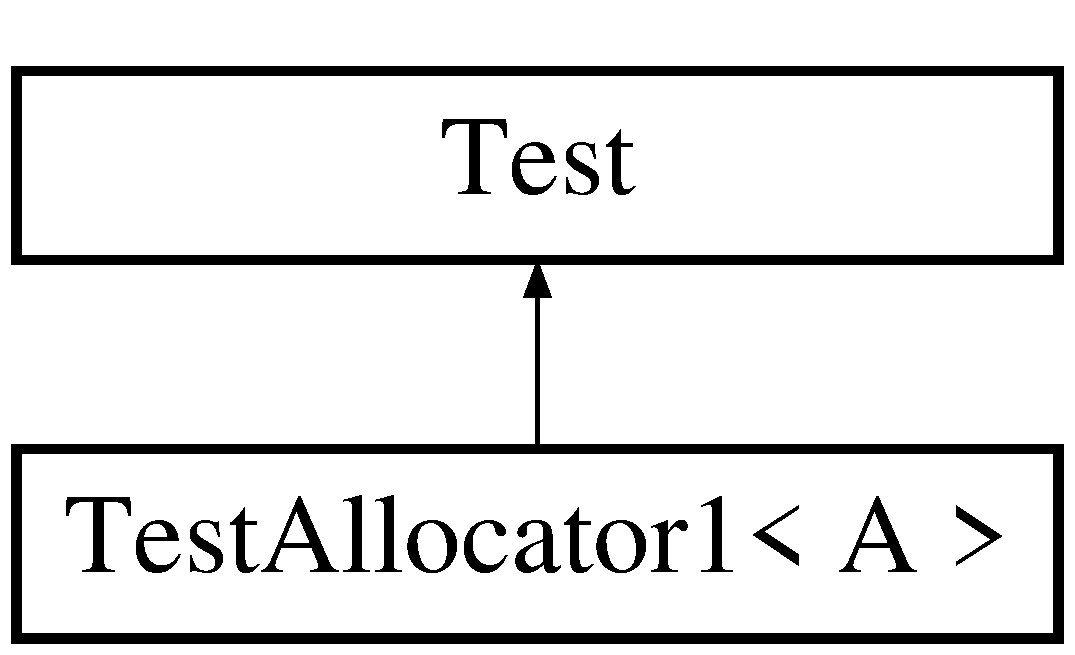
\includegraphics[height=2.000000cm]{structTestAllocator1}
\end{center}
\end{figure}
\subsection*{Public Types}
\begin{DoxyCompactItemize}
\item 
\hypertarget{structTestAllocator1_af833c587251c56fda9cc1169d40545d5}{typedef A {\bfseries allocator\-\_\-type}}\label{structTestAllocator1_af833c587251c56fda9cc1169d40545d5}

\item 
\hypertarget{structTestAllocator1_a92fce0c8423cac5757d6b1d253d646d5}{typedef A\-::value\-\_\-type {\bfseries value\-\_\-type}}\label{structTestAllocator1_a92fce0c8423cac5757d6b1d253d646d5}

\item 
\hypertarget{structTestAllocator1_aa8c669c72a5405cad2024cb1f2d0213d}{typedef A\-::size\-\_\-type {\bfseries size\-\_\-type}}\label{structTestAllocator1_aa8c669c72a5405cad2024cb1f2d0213d}

\item 
\hypertarget{structTestAllocator1_a2d4b518664da974c318e96f1d5fe8cf5}{typedef A\-::pointer {\bfseries pointer}}\label{structTestAllocator1_a2d4b518664da974c318e96f1d5fe8cf5}

\end{DoxyCompactItemize}


The documentation for this struct was generated from the following file\-:\begin{DoxyCompactItemize}
\item 
Test\-Allocator.\-c++\end{DoxyCompactItemize}

\hypertarget{structTestAllocator3}{\section{Test\-Allocator3$<$ A $>$ Struct Template Reference}
\label{structTestAllocator3}\index{Test\-Allocator3$<$ A $>$@{Test\-Allocator3$<$ A $>$}}
}
Inheritance diagram for Test\-Allocator3$<$ A $>$\-:\begin{figure}[H]
\begin{center}
\leavevmode
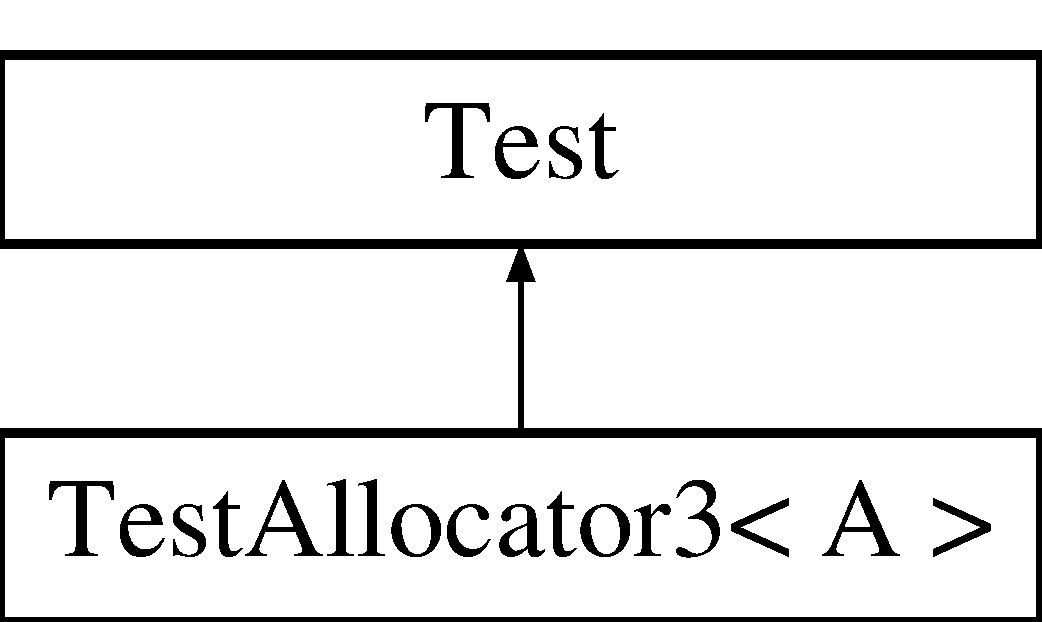
\includegraphics[height=2.000000cm]{structTestAllocator3}
\end{center}
\end{figure}
\subsection*{Public Types}
\begin{DoxyCompactItemize}
\item 
\hypertarget{structTestAllocator3_a2cbf292b14532b741aa9c2d29603cecd}{typedef A {\bfseries allocator\-\_\-type}}\label{structTestAllocator3_a2cbf292b14532b741aa9c2d29603cecd}

\item 
\hypertarget{structTestAllocator3_ac5054dfad63609102029f3bda09f70fc}{typedef A\-::value\-\_\-type {\bfseries value\-\_\-type}}\label{structTestAllocator3_ac5054dfad63609102029f3bda09f70fc}

\item 
\hypertarget{structTestAllocator3_a123816b6d7f35344795ee12a478658d8}{typedef A\-::size\-\_\-type {\bfseries size\-\_\-type}}\label{structTestAllocator3_a123816b6d7f35344795ee12a478658d8}

\item 
\hypertarget{structTestAllocator3_a1e00e0a73b38d61279e77535325b2124}{typedef A\-::pointer {\bfseries pointer}}\label{structTestAllocator3_a1e00e0a73b38d61279e77535325b2124}

\end{DoxyCompactItemize}


The documentation for this struct was generated from the following file\-:\begin{DoxyCompactItemize}
\item 
Test\-Allocator.\-c++\end{DoxyCompactItemize}

%--- End generated contents ---

% Index
\newpage
\phantomsection
\addcontentsline{toc}{chapter}{Index}
\printindex

\end{document}
